\documentclass[a4paper,9pt]{beamer}
\usetheme{Malmoe}  % Now it's a beamer presentation with the lisa theme!
\setbeamertemplate{footline}[page number]
\usecolortheme{beaver}
\usepackage[utf8]{inputenc}
\usepackage{url}
\usepackage{minted}

\usepackage[T1]{fontenc}
\usepackage{inconsolata}

% for copy-pastable ', we need the following
\usepackage{upquote}
\usepackage{textcomp}

%\usepackage{ragged2e}
%\usepackage{multirow}
%\usepackage{fancyvrb}
%\usepackage{color}
\def\imagetop#1{\vtop{\null\hbox{#1}}}

%\logo{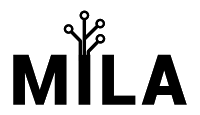
\includegraphics[width=.8in]{mila.png}}
% Standard LaTeX stuff - note the optional abbreviated title being provided

%% ALL that presentation slide are not used! We use a normal frame for that.
\title[Intro to Theano]{Introduction to Theano}
\subtitle{A Fast Python Library for Modelling and Training}
\author[LISA lab]{Pascal Lamblin \\
Institut des algorithmes d'apprentissage de Montréal\\
Montreal Institute for Learning Algorithms\\
Université de Montréal}

\date{%
August 4th, Deep Learning Summer School 2015, Montréal
}

\setbeamertemplate{navigation symbols}{}


\begin{document}

\begin{frame}[plain]
  \titlepage
  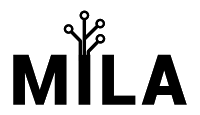
\includegraphics[width=.8in]{mila.png}
  \hfill
  
\includegraphics[width=1in]{UdeM_logo.pdf}
\end{frame}

\section{Overview}
\begin{frame}
  \tableofcontents[currentsection]
\end{frame}

\subsection{Programming Tutorials}

\begin{frame}{Objectives}
  These tutorials should be the occasion for you to:
  \begin{itemize}
    \item Learn about software tools to implement deep learning algorithms
    \item Get some hand-on experience with these tools
    \item Play with simple implementation of existing algorithms
    \item Ask questions and get help from developers and researchers
  \end{itemize}

  \url{http://github.com/mila-udem/summerschool2015/}
\end{frame}


\begin{frame}{Tutorials Schedule}

  \uncover<1->{
      \begin{columns}
        \begin{column}{.07\textwidth}
          
\includegraphics[width=\columnwidth]{lamblinp.jpg}\\
        \end{column}
        \begin{column}{.07\textwidth}
        \end{column}
        \begin{column}{.8\textwidth}
          \scriptsize
          Tuesday, August 4th (day 2)
          \begin{itemize}
            \item Introduction to Theano, Theano examples (Pascal Lamblin)
          \end{itemize}
          \vspace{2mm}
        \end{column}
      \end{columns}
    }

    \uncover<2->{
      \begin{columns}
        \begin{column}{.14\textwidth}
          
\includegraphics[width=\columnwidth]{nvidia-logo.png}\\
        \end{column}
        \begin{column}{.01\textwidth}
        \end{column}
        \begin{column}{.8\textwidth}
          \scriptsize
          Wednesday, August 5th (day 3)
          \begin{itemize}
            \item GPU programming (NVIDIA)
          \end{itemize}
          \vspace{2mm}
        \end{column}
      \end{columns}
    }

    \uncover<3->{
      \begin{columns}
        \begin{column}{.07\textwidth}
          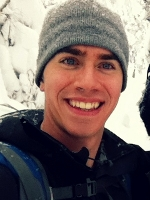
\includegraphics[width=\columnwidth]{dumouliv.jpg}\\
        \end{column}
        \begin{column}{.07\textwidth}
          
\includegraphics[width=\columnwidth]{lamblinp.jpg}\\
        \end{column}
        \begin{column}{.8\textwidth}
          \scriptsize
          Friday, August 7th (day 5)
          \begin{itemize}
            \item Fuel: a library for machine learning datasets (Vincent Dumoulin)
            \item Deep neural networks in Theano (Pascal Lamblin)
          \end{itemize}
          \vspace{2mm}
        \end{column}
      \end{columns}
    }

    \uncover<4->{
      \begin{columns}
        \begin{column}{.07\textwidth}
          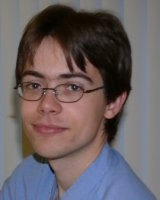
\includegraphics[width=\columnwidth]{fred_lisa2.jpg}
        \end{column}
        \begin{column}{.07\textwidth}
          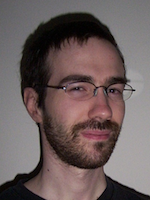
\includegraphics[width=\columnwidth]{abergeron.png}
        \end{column}
        \begin{column}{.8\textwidth}
          \scriptsize
          Monday, August 10th (day 8)
          \begin{itemize}
            \item Debugging with Theano (Frédéric Bastien)
            \item Convolutional networks (Arnaud Bergeron)
          \end{itemize}
          \vspace{2mm}
        \end{column}
      \end{columns}
    }

    \uncover<5->{
      \begin{columns}
        \begin{column}{.07\textwidth}
          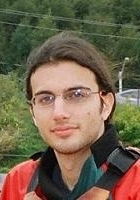
\includegraphics[width=\columnwidth]{carriepl.jpg}
        \end{column}
        \begin{column}{.07\textwidth}
          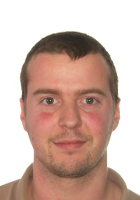
\includegraphics[width=\columnwidth]{philemon_brakel.jpg}
        \end{column}
        \begin{column}{.8\textwidth}
          \scriptsize
          Tuesday, August 11th (day 9)
          \begin{itemize}
            \item Scan: Loops in Theano (Pierre Luc Carrier)
            \item Recurrent neural networks (Philémon Brakel)
          \end{itemize}
          \vspace{2mm}
        \end{column}
      \end{columns}
    }

    \uncover<6->{
      \begin{columns}
        \begin{column}{.07\textwidth}
        \end{column}
        \begin{column}{.07\textwidth}
        \end{column}
        \begin{column}{.8\textwidth}
          \scriptsize
          Wednesday, August 12th (day 10)
          \begin{itemize}
            \item Overflow session
          \end{itemize}
          \vspace{2mm}
        \end{column}
      \end{columns}
    }

\end{frame}

\subsection{Motivation}
%TODO: TOC, current section

\begin{frame}{Theano vision}

  Mathematical symbolic expression compiler

  \begin{itemize}
    \item Easy to define expressions
      \begin{itemize}
        \item Expressions mimic NumPy's syntax and semantics
      \end{itemize}
    \item Possible to manipulate those expressions
      \begin{itemize}
        \item Substitutions
        \item Gradient, R operator
        \item Stability optimizations
      \end{itemize}
    \item Fast to compute values for those expressions
      \begin{itemize}
        \item Speed optimizations
        \item Use fast back-ends (CUDA, BLAS, custom C code)
      \end{itemize}
    \item Tools to inspect and check for correctness
  \end{itemize}
\end{frame}

\begin{frame}[fragile]{Current status}
  \begin{itemize}
    \item Mature: Theano has been developed and used since January 2008 (7 yrs old)
    \item Driven hundreds of research papers
    \item Good user documentation
    \item Active mailing list with participants worldwide
    \item Core technology for Silicon Valley start-ups
    \item Many contributors from different places
    \item Used to teach university classes
    \item Has been used for research at large companies
  \end{itemize}
  Theano: \url{deeplearning.net/software/theano/}

  Deep Learning Tutorials: \url{deeplearning.net/tutorial/}
\end{frame}

\begin{frame}{Related projects}
  Many libraries ar build on top of Theano (mostly machine learning)
  \begin{itemize}
  \item Pylearn2
  \item Blocks
  \item PyMC 3
  \item PyAutoDiff
  \item Lasagne
  \item sklearn-theano
  \item theano-rnn
  \item Morb
  \item Keras
  \item \ldots
  \end{itemize}
\end{frame}


\subsection{Basic Usage}
\begin{frame}{Basic usage}
  Theano defines a {\bf language}, a {\bf compiler}, and a {\bf library}.
  \begin{itemize}
    \item Define a symbolic expression
    \item Compile a function that can compute values
    \item Execute that function on numeric values
  \end{itemize}
\end{frame}

\begin{frame}[fragile]{Defining an expression}
  \begin{itemize}
    \item Symbolic, strongly-typed inputs
      \begin{minted}[fontfamily=tt]{python}
import theano
from theano import tensor as T
x = T.vector('x')
W = T.matrix('W')
b = T.vector('b')
    \end{minted}
    \item NumPy-like syntax to build expressions
      \begin{minted}{python}
dot = T.dot(x, W)
out = T.nnet.sigmoid(dot + b)
      \end{minted}
  \end{itemize}
\end{frame}

\begin{frame}[fragile]{Graph visualization (1)}
  \begin{verbatim}
debugprint(dot)
dot [@A] ''   
 |x [@B]
 |W [@C]

debugprint(out)
sigmoid [@A] ''   
 |Elemwise{add,no_inplace} [@B] ''   
   |dot [@C] ''   
   | |x [@D]
   | |W [@E]
   |b [@F]
  \end{verbatim}
\end{frame}

\begin{frame}[fragile]{Compiling a Theano function}
  Build a callable that compute outputs given inputs
  \begin{minted}{python}
f = theano.function(inputs=[x, W], outputs=dot)
g = theano.function([x, W, b], out)
h = theano.function([x, W, b], [dot, out])
i = theano.function([x, W, b], [dot + b, out])
  \end{minted}
\end{frame}

\begin{frame}[fragile]{Graph visualization (2)}
  \begin{columns}
    \begin{column}{0.48\textwidth}
\footnotesize
      \begin{verbatim}
theano.printing.debugprint(f)
CGemv{inplace} [@A] ''   3
 |Alloc [@B] ''   2
 | |TensorConstant{0.0} [@C]
 | |Shape_i{1} [@D] ''   1
 |   |W [@E]
 |TensorConstant{1.0} [@F]
 |InplaceDimShuffle{1,0} [@G] 'W.T'   0
 | |W [@E]
 |x [@H]
 |TensorConstant{0.0} [@C]

theano.printing.pydotprint(f)
      \end{verbatim}
    \end{column}
    \begin{column}{0.48\textwidth}
\footnotesize
      \begin{verbatim}
theano.printing.debugprint(g)
Elemwise{ScalarSigmoid}[(0, 0)] [@A] ''   2
 |CGemv{no_inplace} [@B] ''   1
   |b [@C]
   |TensorConstant{1.0} [@D]
   |InplaceDimShuffle{1,0} [@E] 'W.T'   0
   | |W [@F]
   |x [@G]
   |TensorConstant{1.0} [@D]

theano.printing.pydotprint(g)
      \end{verbatim}
    \end{column}
  \end{columns}
\end{frame}

\begin{frame}{\tt pydotprint(f)}
    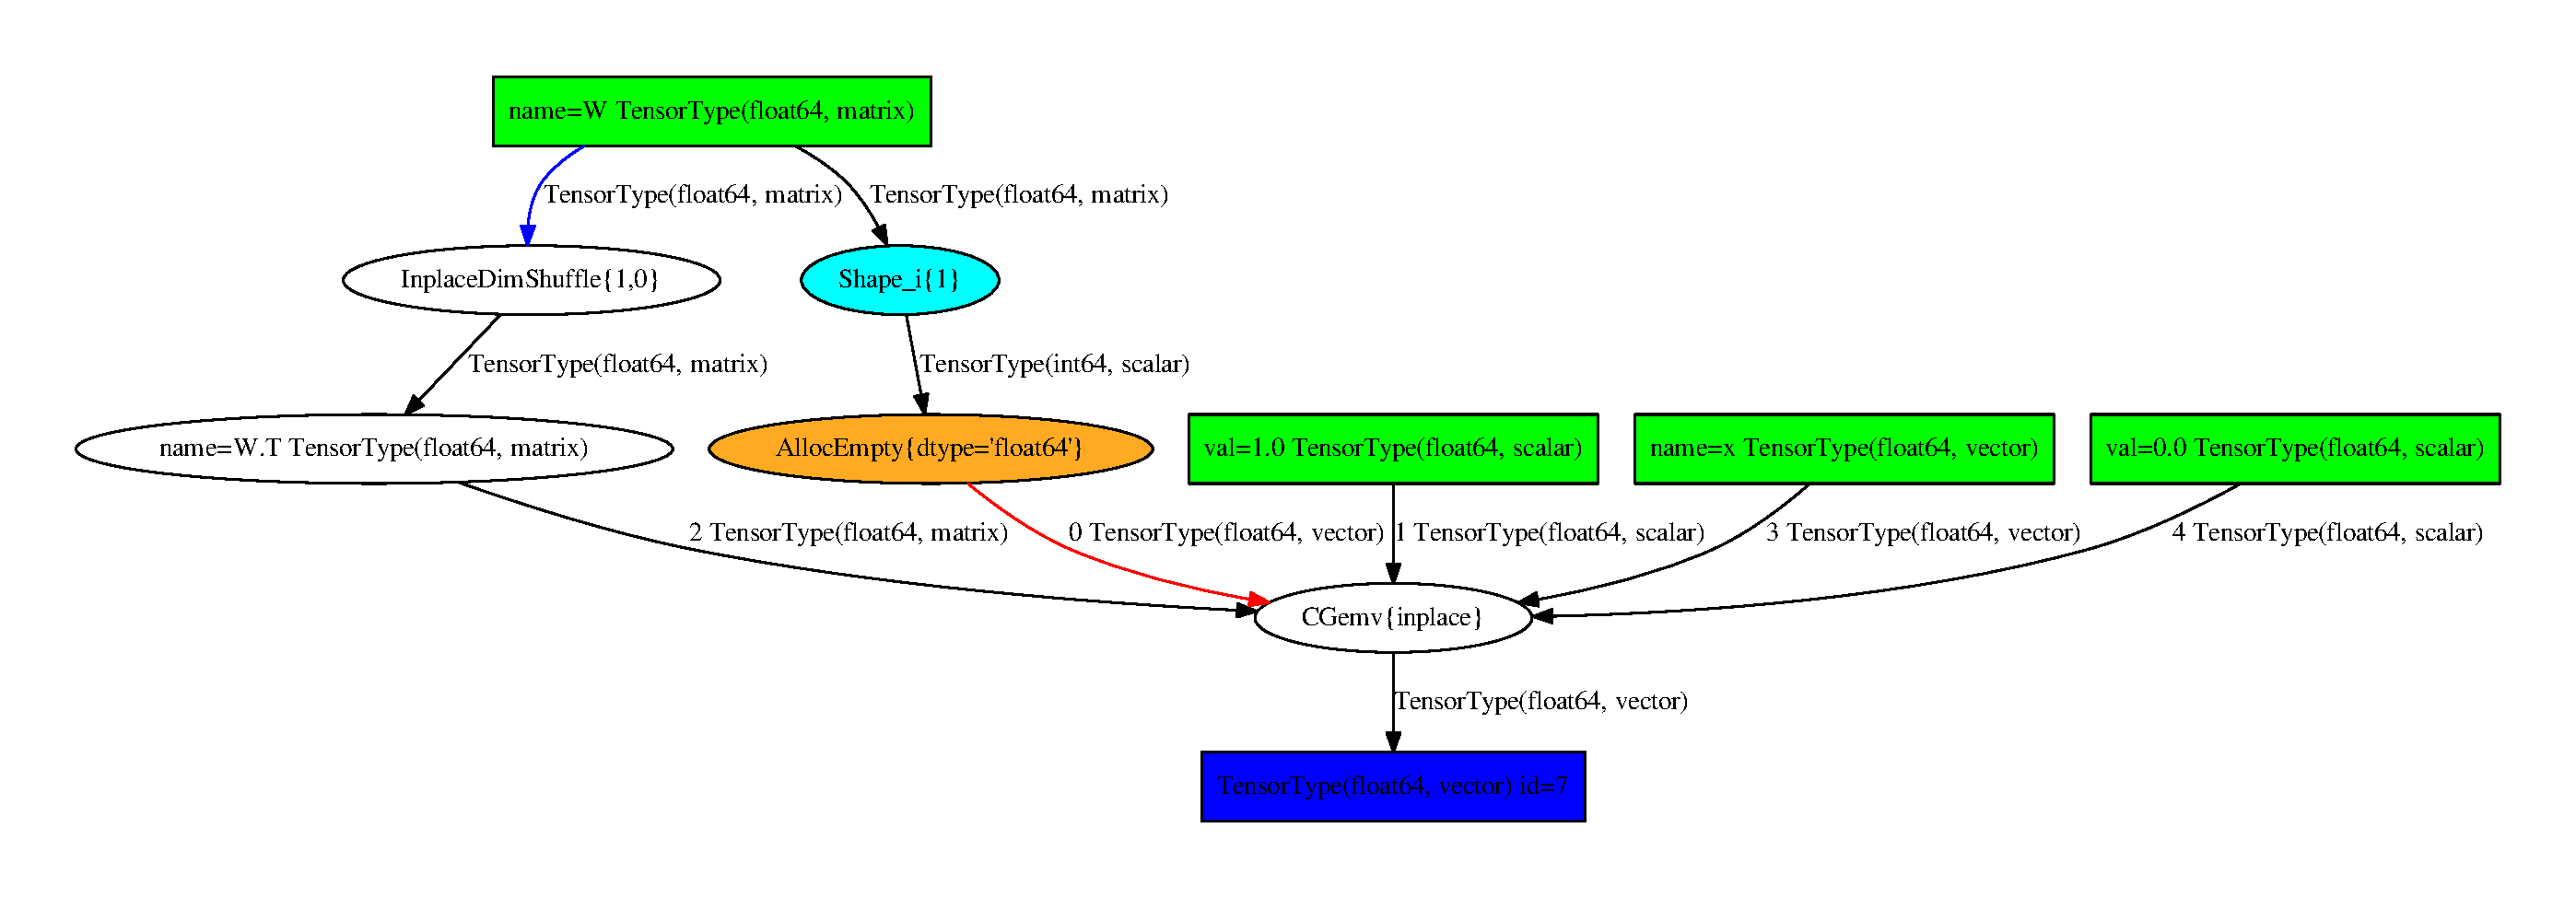
\includegraphics[width=\textwidth]{pydotprint_f.pdf}
\end{frame}
\begin{frame}{\tt pydotprint(g)}
    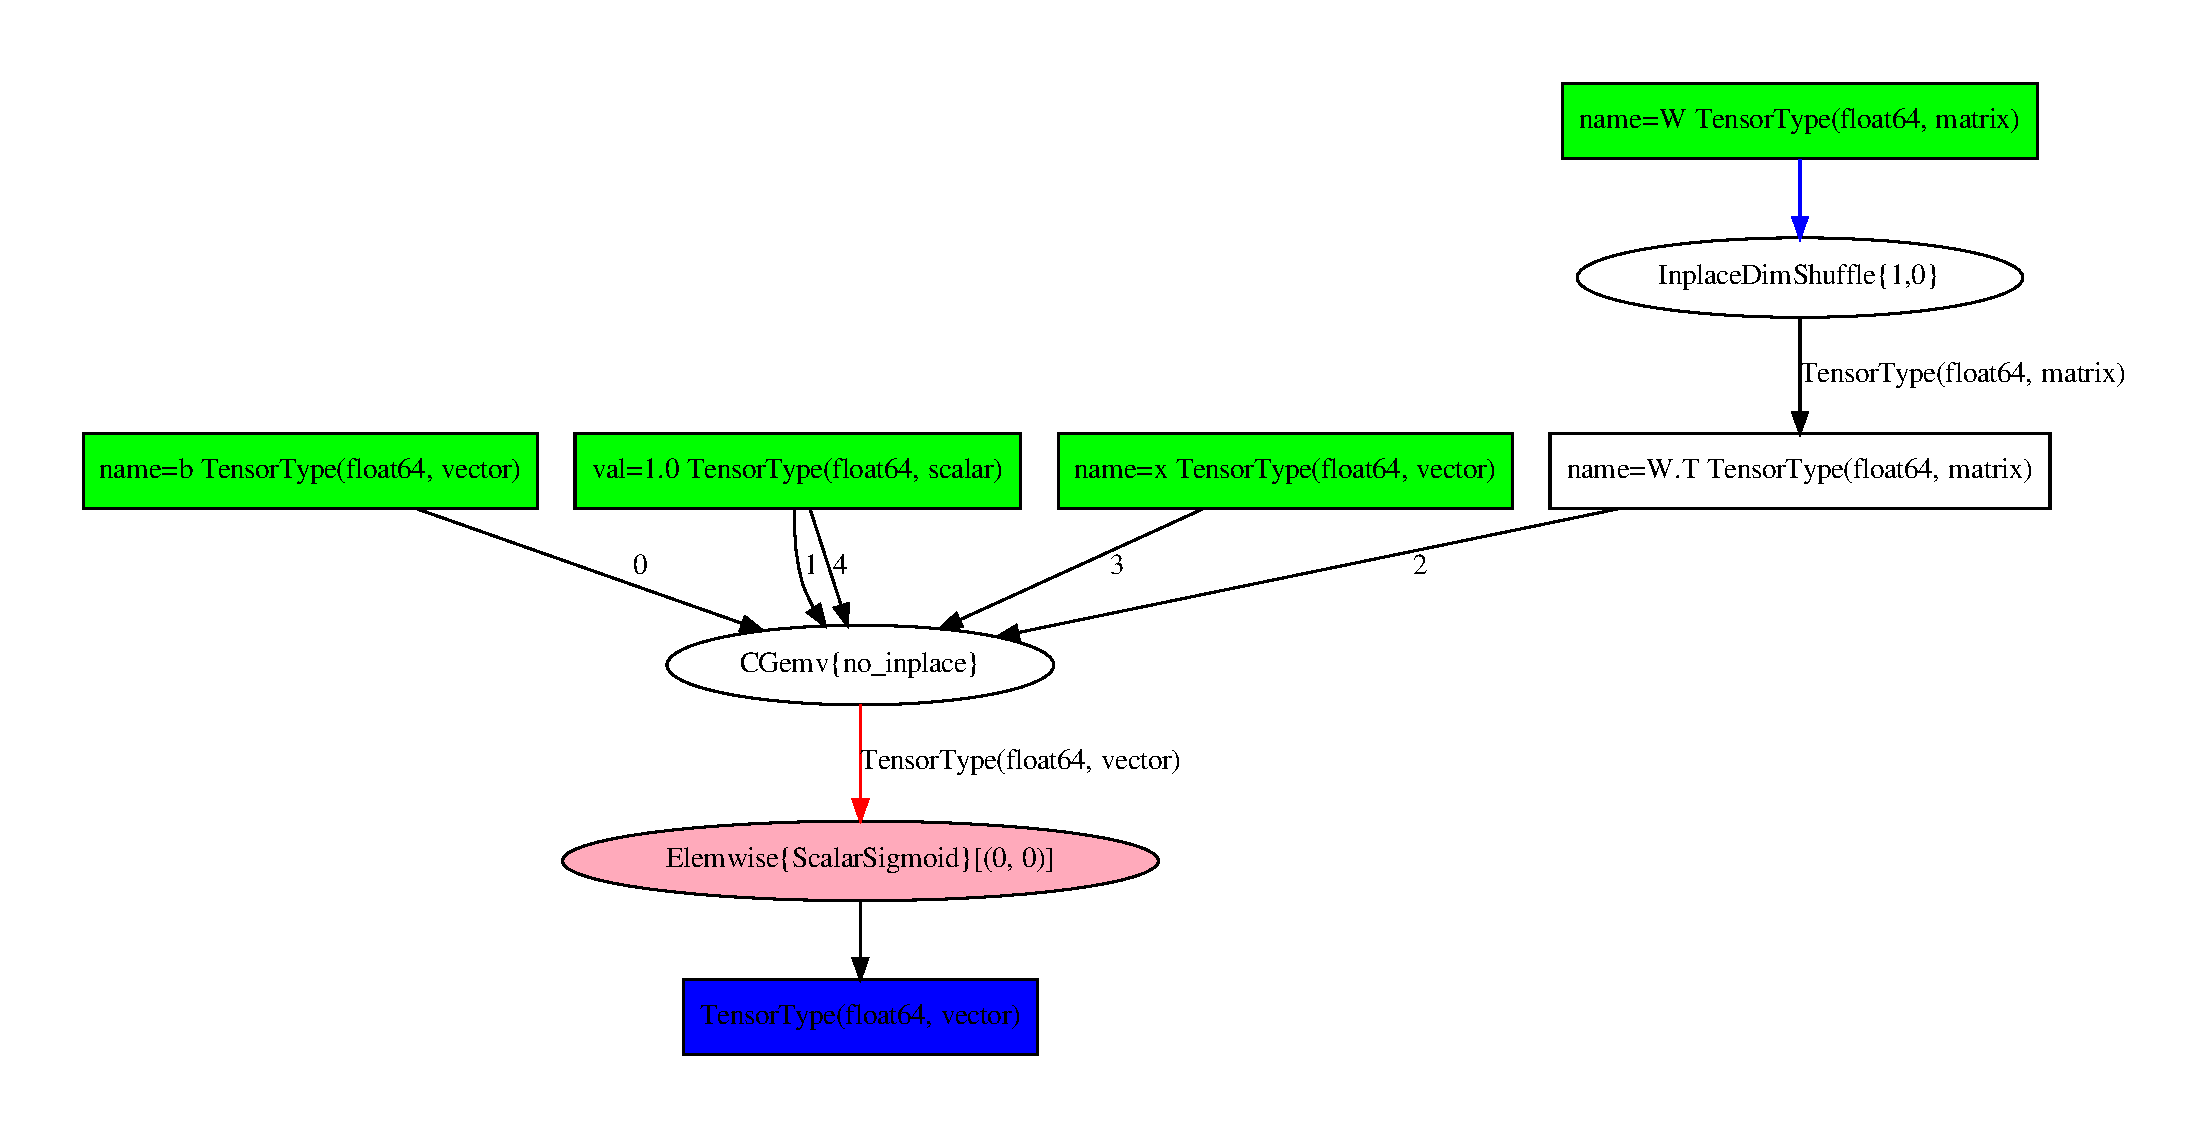
\includegraphics[width=\textwidth]{pydotprint_g.pdf}
\end{frame}
\begin{frame}{\tt pydotprint(h)}
    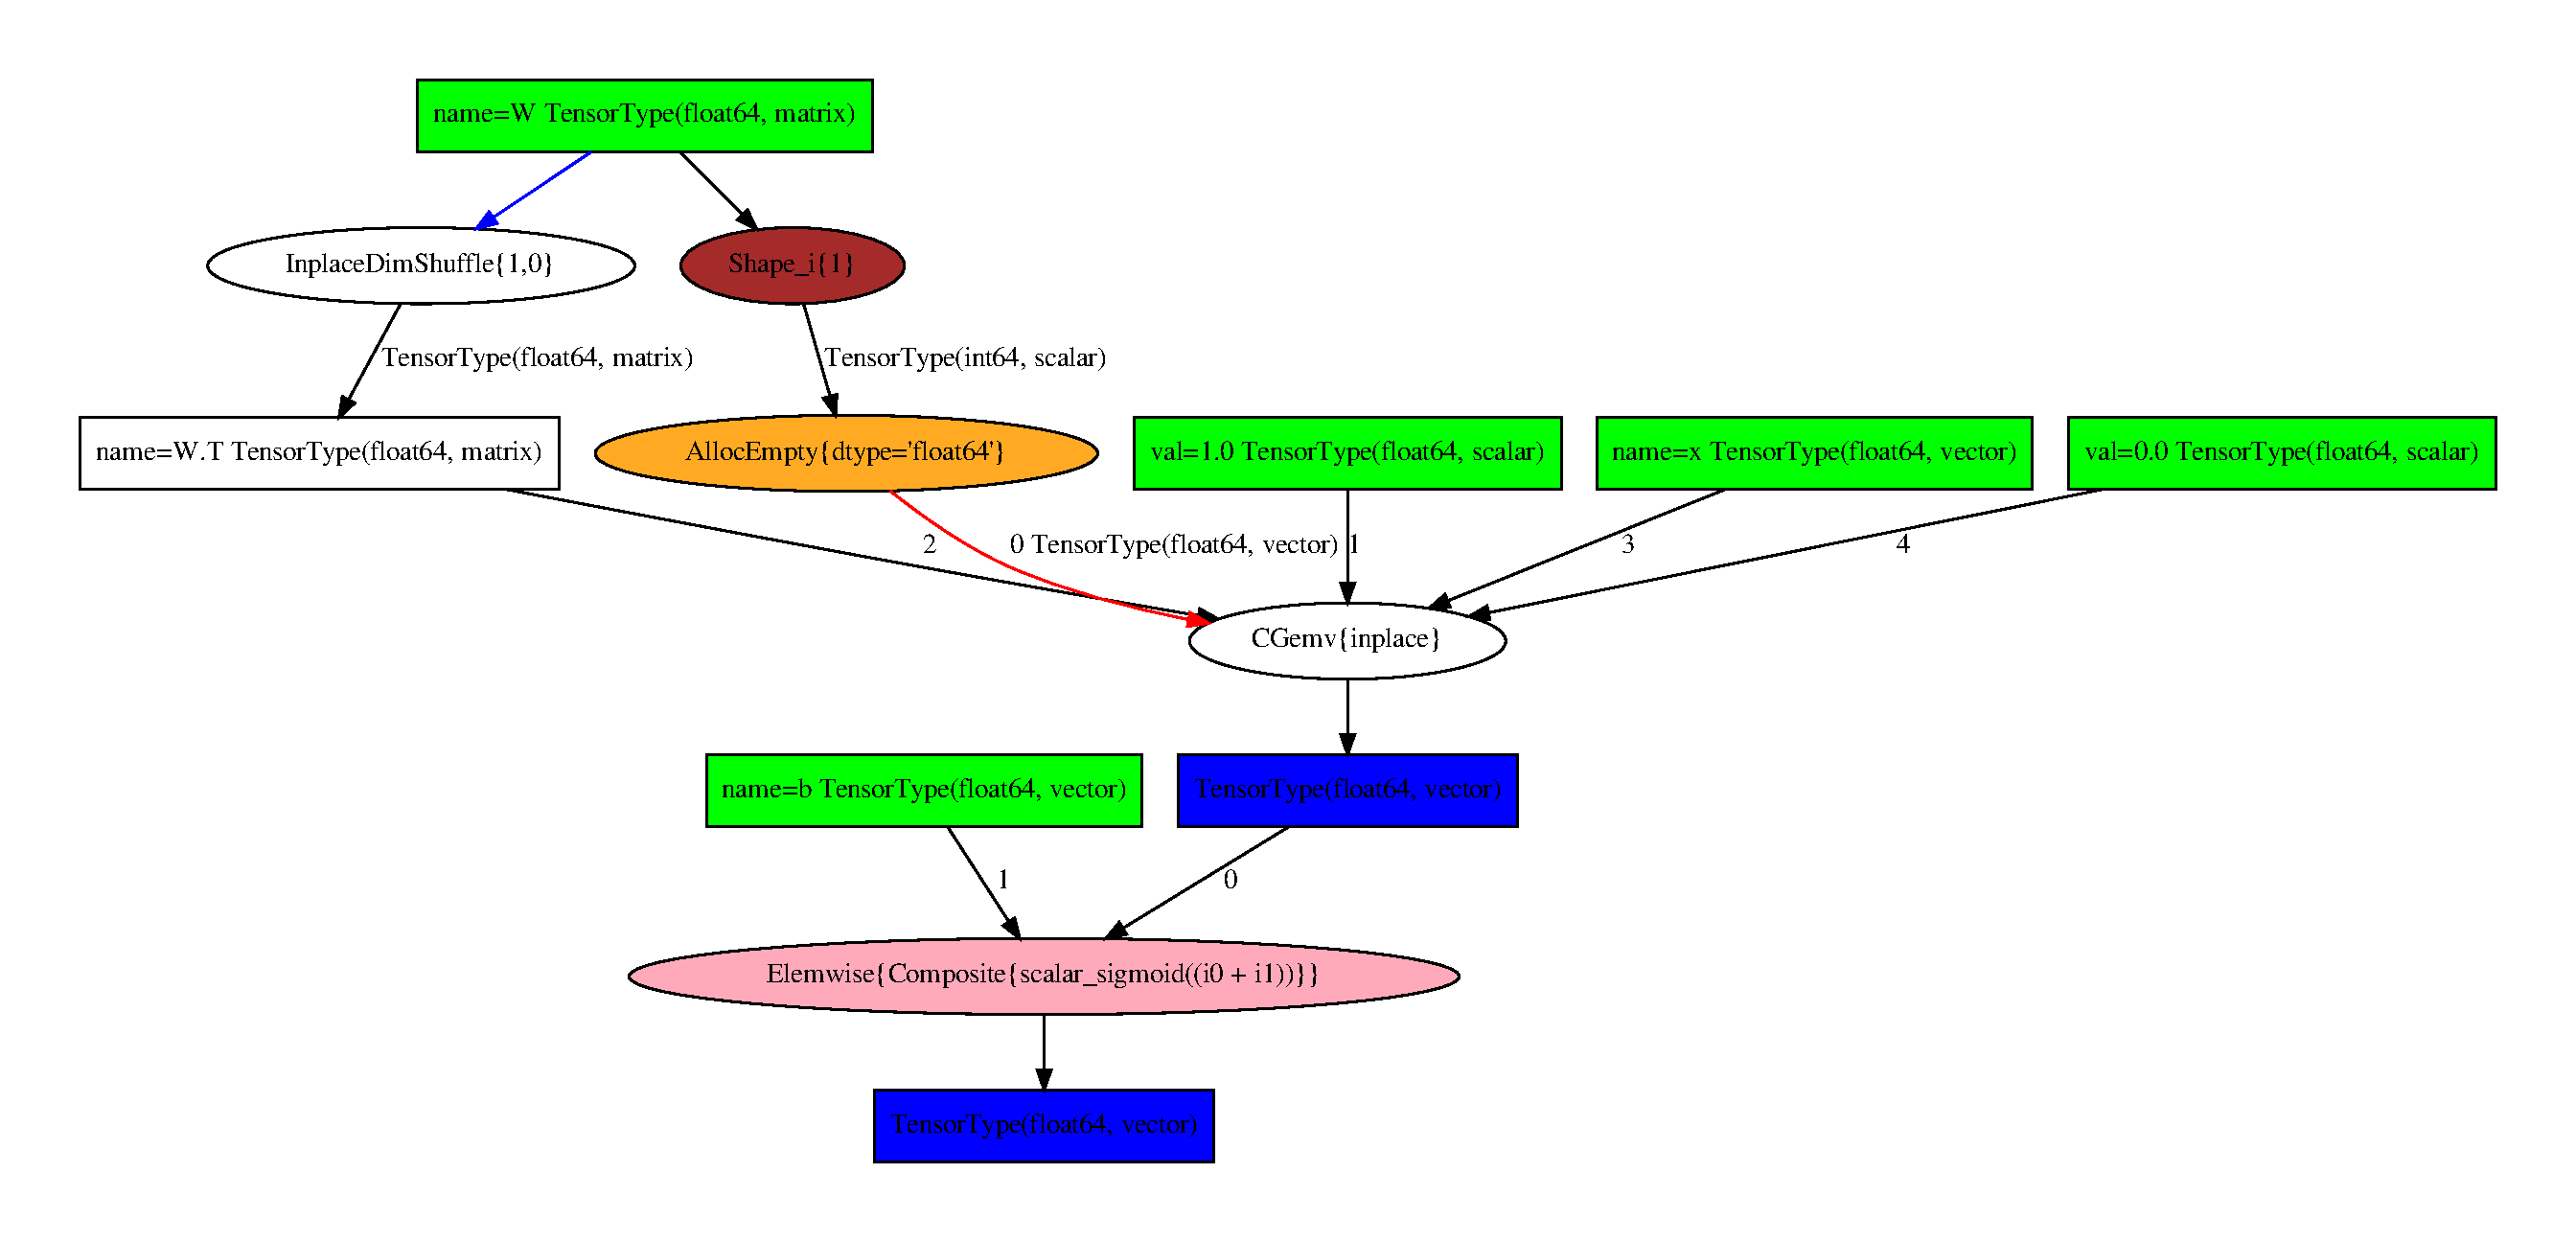
\includegraphics[width=\textwidth]{pydotprint_h.pdf}
\end{frame}

\begin{frame}[fragile]{Executing a Theano function}
  Call it with numeric values
\small
  \begin{minted}{python}
import numpy as np
np.random.seed(42)
W_val = np.random.randn(4, 3)
x_val = np.random.rand(4)
b_val = np.ones(3)

f(x_val, W_val)
# -> array([ 1.79048354,  0.03158954, -0.26423186])

g(x_val, W_val, b_val)
# -> array([ 0.9421594 ,  0.73722395,  0.67606977])

h(x_val, W_val, b_val)
# -> [array([ 1.79048354,  0.03158954, -0.26423186]),
#     array([ 0.9421594 ,  0.73722395,  0.67606977])]

i(x_val, W_val, b_val)
# -> [array([ 2.79048354,  1.03158954,  0.73576814]),
#     array([ 0.9421594 ,  0.73722395,  0.67606977])]
  \end{minted}
\end{frame}

\section{Graph definition and Syntax}
\begin{frame}
  \tableofcontents[currentsection]
\end{frame}
\subsection{Strong typing}
\begin{frame}{Strong typing}
  \begin{itemize}
    \item All Theano variables have a type
    \item Different categories of types. Most used:
      \begin{itemize}
        \item TensorType for NumPy ndarrays
        \item CudaNdarrayType for CUDA arrays
        \item Sparse for scipy.sparse matrices
      \end{itemize}
    \item ndim, dtype, broadcastable pattern are part of the type
    \item shape and memory layout (strides) are {\bf not}
  \end{itemize}
\end{frame}

\begin{frame}[fragile]{Broadcasting tensors}
  \begin{itemize}
    \item Implicit replication of arrays along broadcastable dimensions
    \item Broadcastable dimensions will {\bf always} have length 1
    \item Such dimensions can be added to the left
  \end{itemize}
  \begin{minted}{python}
r = T.row('r')
print(r.broadcastable)  # (True, False)
c = T.col('c')
print(c.broadcastable)  # (False, True)

f = theano.function([r, c], r + c)
print(f([[1, 2, 3]], [[.1], [.2]]))
  \end{minted}
\end{frame}

\subsection{Differences from Python/NumPy}
\begin{frame}[fragile]{No side effects}
  Create new variables, cannot {\em change} them
  \begin{itemize}
    \item \verb|a += 1| works, returns new variable and re-assign
    \item \verb|a[:] += 1|, or \verb|a[:] = 0| do {\bf not} work
      (the \verb|__setitem__| method cannot return a new object)
    \item \verb|a = T.inc_subtensor(a[:], 1)| or \verb|a = T.set_subtensor(a[:], 0)|
    \item This will create a new variable, and re-assign a to it
    \item Theano will figure out later if it can use an in-place version
  \end{itemize}
  Exceptions:
  \begin{itemize}
    \item The \verb|Print()| Op
    \item The \verb|Assert()| Op
    \item You have to re-assign (or use the returned value)
    \item These can disrupt some optimizations
      %TODO: example
  \end{itemize}
\end{frame}

\begin{frame}[fragile]{Python keywords}
  We cannot redefine Python's keywords: they affect the flow when building the graph, not when executing it.
  \begin{itemize}
    \item \verb|if var:| will always evaluate to \verb|True|.
      Use \verb|theano.ifelse.ifelse(var, expr1, expr2)|
    \item \verb|for i in var:| will not work if \verb|var| is symbolic.
      If \verb|var| is numeric: loop unrolling. You can use \verb|theano.scan|.
    \item \verb|len(var)| cannot return a symbolic shape, you can use
      \verb|var.shape[0]|
    \item \verb|print| will print an identifier for the symbolic variable,
      there is a \verb|Print()| operation
  \end{itemize}
\end{frame}


\section{Graph Transformations}
\begin{frame}
  \tableofcontents[currentsection]
\end{frame}

\subsection{Substitution and Cloning}
\begin{frame}[fragile]{The {\tt givens} keyword}
  Substitution at the last moment, when compiling a function
  \begin{minted}{python}
x_ = T.vector('x_')
x_n = (x_ - x_.mean()) / x_.std()
f_n = theano.function([x_, W], dot, givens={x: x_n})
f_n(x_val, W_val)
# -> array([ 1.90651511,  0.60431744, -0.64253361])
  \end{minted}
\end{frame}

\begin{frame}[fragile]{Cloning with replacement}
  Useful when building the expression graph
  \begin{minted}{python}
dot_n, out_n = theano.clone(
    [dot, out],
    replace={x: (x - x.mean()) / x.std()})
f_n = theano.function([x, W], dot_n)
f_n(x_val, W_val)
# -> array([ 1.90651511,  0.60431744, -0.64253361])
  \end{minted}
\end{frame}

\subsection{Gradient}
\begin{frame}{The back-propagation algorithm}
  Application of the chain-rule for functions from ${\mathbb R}^N$ to ${\mathbb R}$.
  \begin{itemize}
    \item $C: {\mathbb R}^N \rightarrow {\mathbb R}$
    \item $f: {\mathbb R}^M \rightarrow {\mathbb R}$
    \item $g: {\mathbb R}^N \rightarrow {\mathbb R}^M$
    \item $C(x) = f(g(x))$
    \item $\left.\frac{\partial C}{\partial x}\right|_x =
              \left.\frac{\partial f}{\partial g}\right|_{g(x)}
              \cdot \left.\frac{\partial g}{\partial x}\right|_x$
  \end{itemize}
  The whole $M \times N$ Jacobian matrix $\left.\frac{\partial g}{\partial x}\right|_x$
  is not needed.

  We only need $\nabla g_x: {\mathbb R}^M \rightarrow {\mathbb R}^N, v \mapsto v \cdot \left.\frac{\partial g}{\partial x}\right|_x$
\end{frame}

\begin{frame}[fragile]{Using theano.grad}
  \begin{minted}{python}
y = T.vector('y')
C = ((out - y) ** 2).sum()
dC_dW = theano.grad(C, W)
dC_db = theano.grad(C, b)
# or dC_dW, dC_db = theano.grad(C, [W, b])
  \end{minted}
  \begin{itemize}
    \item \verb|dC_dW| and \verb|dC_db| are symbolic expressions, like \verb|W| and \verb|b|
    \item There are no numerical values at this point
  \end{itemize}
\end{frame}

\begin{frame}[fragile]{Using the gradients}
  \begin{itemize}
    \item The symbolic gradients can be used to build a Theano function
      \begin{minted}{python}
cost_and_grads = theano.function([x, W, b, y], [C, dC_dW, dC_db])
y_val = np.random.uniform(size=3)
print(cost_and_grads(x_val, W_val, b_val, y_val))
      \end{minted}
    \item They can also be used to build new expressions
      \begin{minted}{python}
upd_W = W - 0.1 * dC_dW
upd_b = b - 0.1 * dC_db
cost_and_upd = theano.function([x, W, b, y], [C, upd_W, upd_b])
print cost_and_upd(x_val, W_val, b_val, y_val)
      \end{minted}
  \end{itemize}
\end{frame}

\begin{frame}
  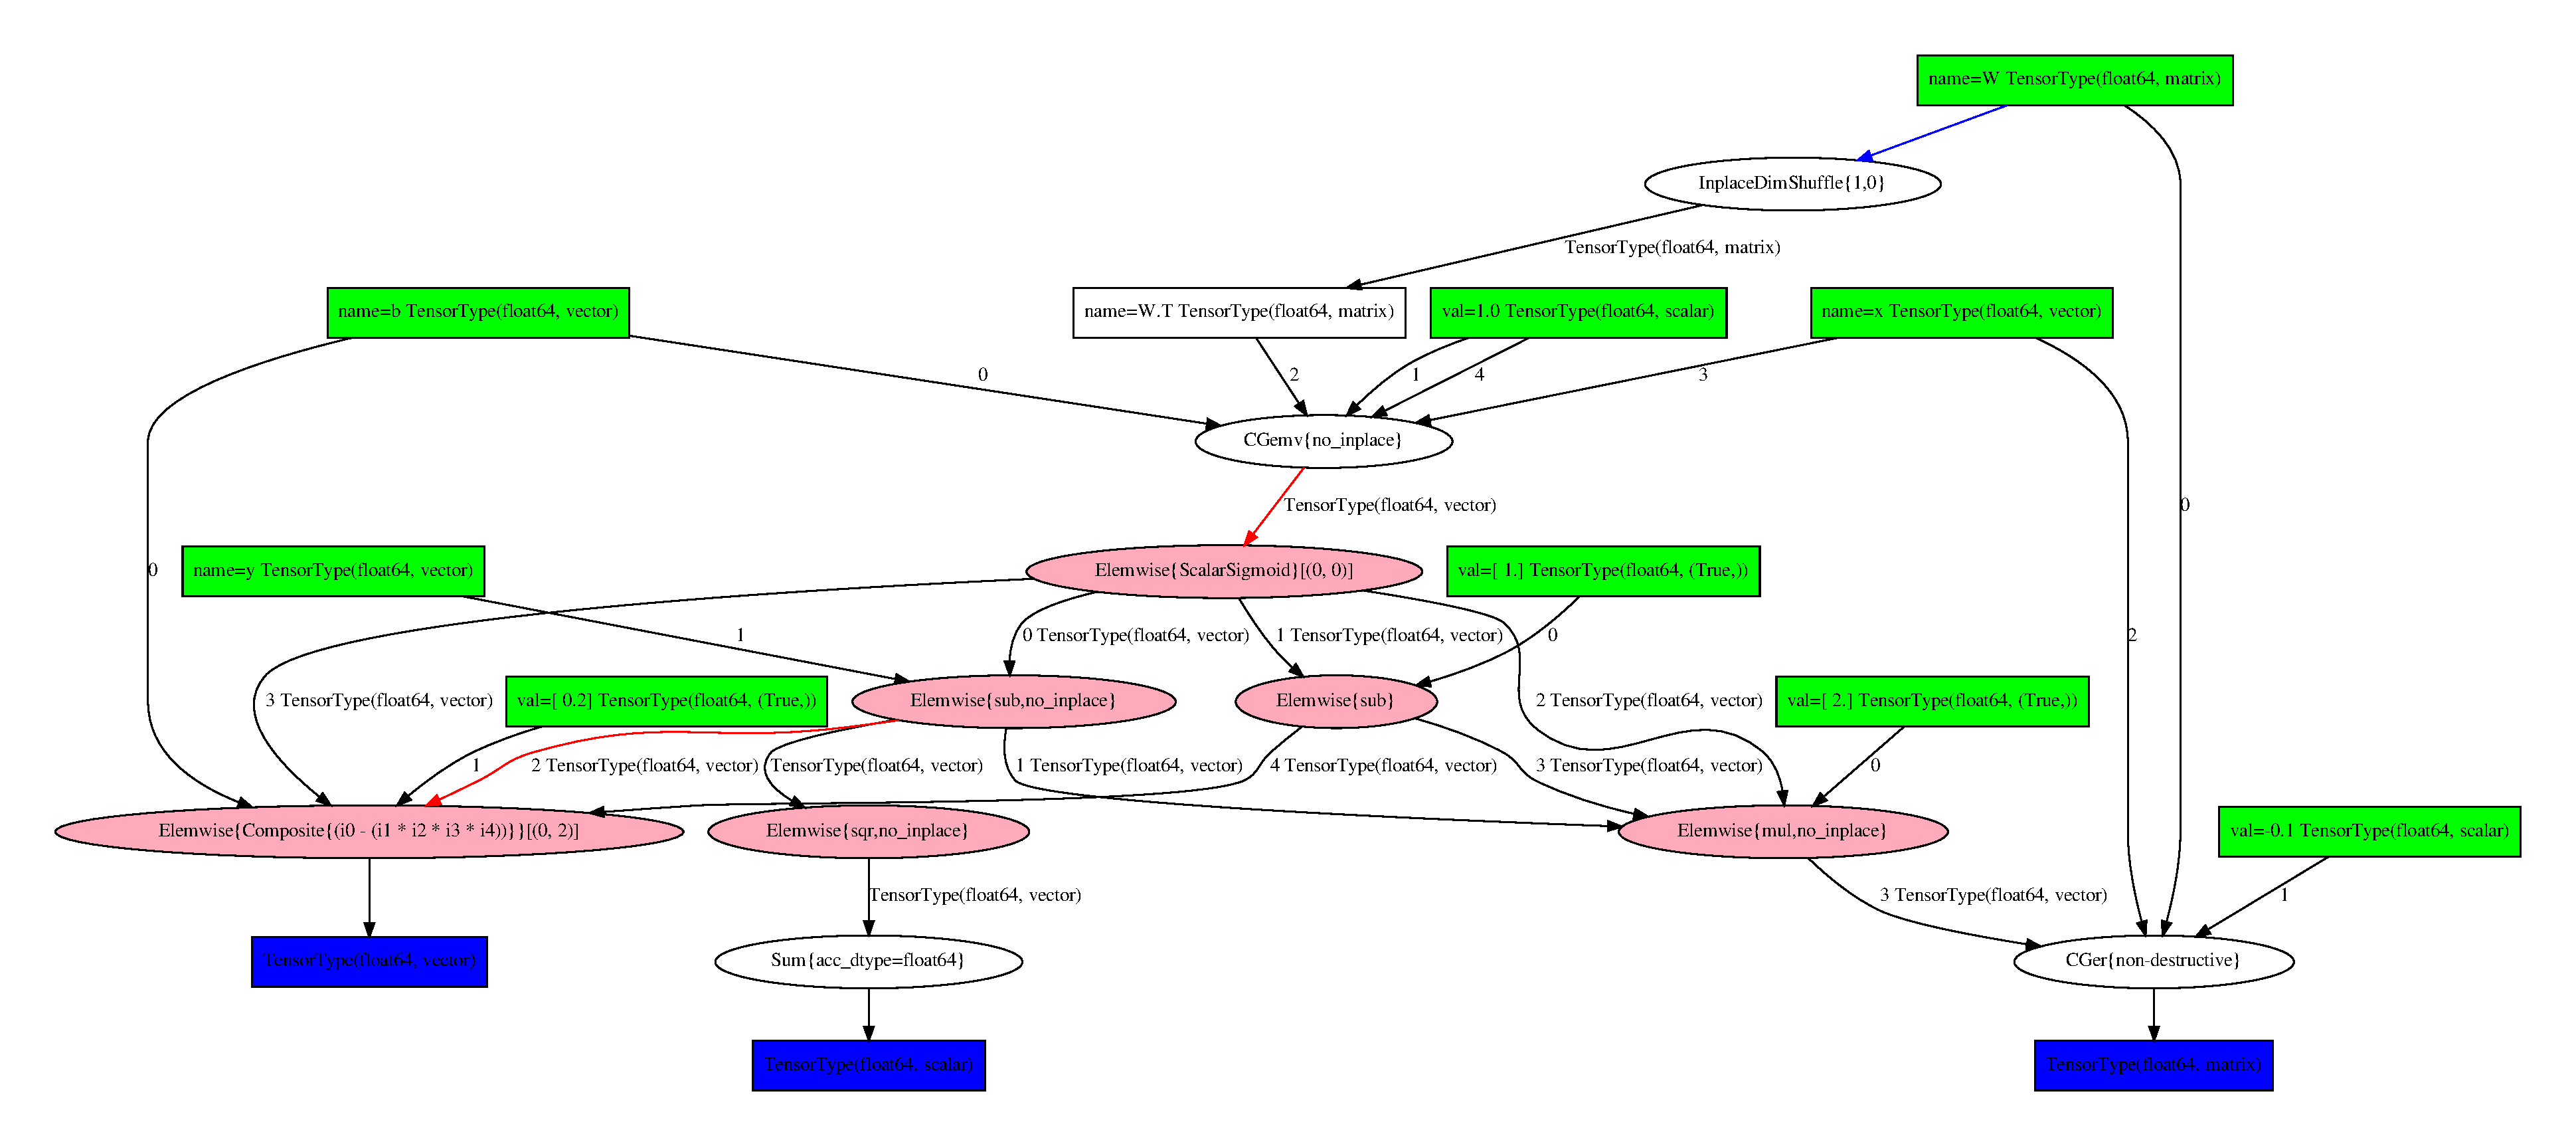
\includegraphics[width=\textwidth]{pydotprint_cost_and_upd.pdf}
\end{frame}

\subsection{Shared variables}
\begin{frame}[fragile]{Update values}
  Simple ways to update values
  \begin{minted}{python}
C_val, dC_dW_val, dC_db_val = cost_and_grads(x_val, W_val, b_val, y_val)
W_val -= 0.1 * dC_dW_val
b_val -= 0.1 * dC_db_val

C_val, W_val, b_val = cost_and_upd(x_val, W_val, b_val, y_val)
  \end{minted}
  \begin{itemize}
    \item Cumbersome
    \item Inefficient: memory, GPU transfers
  \end{itemize}
\end{frame}

\begin{frame}{Shared variables}
  \begin{itemize}
    \item Symbolic variables, with a {\bf value} associated to them
    \item The value is {\bf persistent} across function calls
    \item The value is {\bf shared} among all functions
    \item The variable has to be an {\bf input variable}
    \item The variable is an {\bf implicit input} to all functions using it
  \end{itemize}
\end{frame}

\begin{frame}[fragile]{Using shared variables}
  \begin{minted}{python}
x = T.vector('x')
y = T.vector('y')
W = theano.shared(W_val)
b = theano.shared(b_val)
dot = T.dot(x, W)
out = T.nnet.sigmoid(dot + b)
f = theano.function([x], dot)  # W is an implicit input
g = theano.function([x], out)  # W and b are implicit inputs
print(f(x_val))
# [ 1.79048354  0.03158954 -0.26423186]
print(g(x_val))
# [ 0.9421594   0.73722395  0.67606977]
  \end{minted}
  \begin{itemize}
    \item Use \verb|W.get_value()| and \verb|W.set_value()|
      to access the value later
  \end{itemize}
\end{frame}

\begin{frame}[fragile]{Updating shared variables}
  \begin{minted}{python}
C = ((out - y) ** 2).sum()
dC_dW, dC_db = theano.grad(C, [W, b])
upd_W = W - 0.1 * dC_dW
upd_b = b - 0.1 * dC_db

cost_and_perform_updates = theano.function(
    inputs=[x, y],
    outputs=C,
    updates=[(W, upd_W),
             (b, upd_b)])
  \end{minted}
  \begin{itemize}
    \item Variables \verb|W| and \verb|b| are {\bf implicit inputs}
    \item Expressions \verb|upd_W| and \verb|upd_b| are {\bf implicit outputs}
    \item All outputs, including the update expressions, are computed {\bf before} the updates are performed
  \end{itemize}
\end{frame}

\begin{frame}
  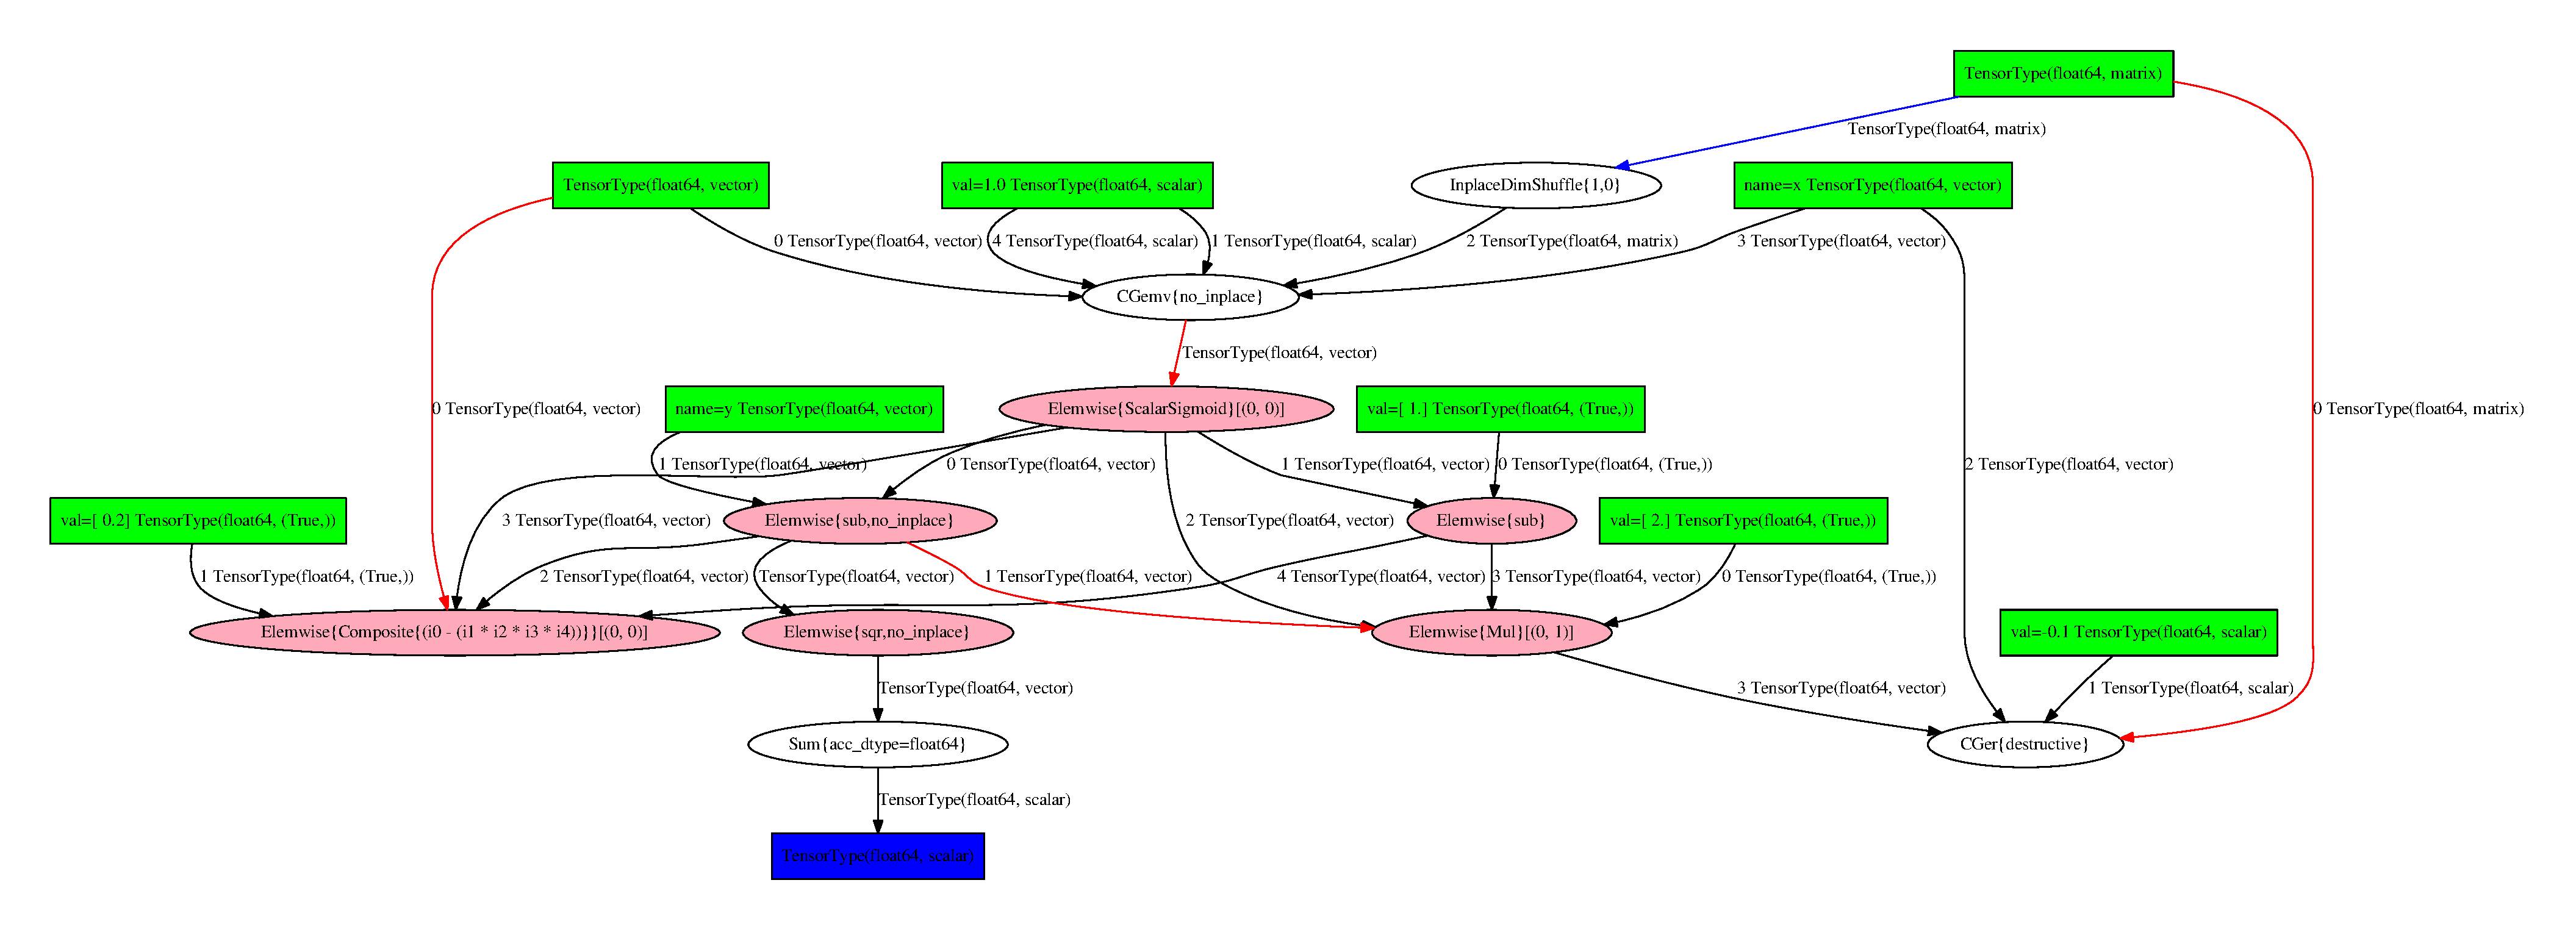
\includegraphics[width=\textwidth]{pydotprint_cost_and_perform_updates.pdf}
\end{frame}


\section{Make it fast!}
\begin{frame}
  \tableofcontents[currentsection]
\end{frame}
\subsection{Optimizations}
\begin{frame}{Graph optimizations}
  An optimization replaces a part of the graph with different nodes
  \begin{itemize}
    \item The types of the replaced nodes have to match
  \end{itemize}
  Different goals for optimizations:
  \begin{itemize}
    \item Merge equivalent computations
    \item Simplify expressions: $x / x$ becomes $1$
    \item Numerical stability: Gives the right answer for ``$\log (1 + x)$'' even if $x$ is really tiny.
    \item Insert in-place an destructive versions of operations
    \item Use specialized, high-performance versions (Elemwise loop fusion, GEMV, GEMM)
    \item Shape inference
    \item Constant folding
    \item Transfer to GPU
  \end{itemize}
\end{frame}

\begin{frame}[fragile]{Enabling/disabling optimizations}
  Trade-off between compilation speed, execution speed, error detection.

  Different modes govern how much optimizations are applied
  \begin{itemize}
    \item \verb|'FAST_RUN'|: default, make the runtime as fast as possible, launching overhead.
      Includes moving computation to GPU if a GPU was selected
    \item \verb|'FAST_COMPILE'|: minimize launching overhead, around NumPy speed
    \item \verb|'DEBUG_MODE'|: checks and double-checks everything, extremely slow
    \item Enable and disable particular optimizations or sets of optimizations
    \item Can be done globally, or for each function
  \end{itemize}
\end{frame}

\subsection{Code Generation}
\begin{frame}[fragile]{C code for Ops}
  \begin{itemize}
    \item Each operator can define C code computing the outputs given the inputs
    \item Otherwise, fall back to a Python implementation
  \end{itemize}
  How does this work?
  \begin{itemize}
    \item In Python, build a string representing the C code for a Python module
    \begin{itemize}
      \item Stitching together code to extract data from Python structure,
      \item Takes into account input and output types (ndim, dtype, \ldots)
      \item String substitution for names of variables
    \end{itemize}
    \item That module is compiled by \verb|g++|
    \item The compiled module gets imported in Python
    \item Versioned cache of generated and compiled C code
  \end{itemize}
  For GPU code, same process, using CUDA and \verb|nvcc| instead.
\end{frame}

\begin{frame}[fragile]{The C virtual machine (CVM)}
  A runtime environment, or VM, that calls the functions performing
  computation of different parts of the function (from inputs to
  outputs)
  \begin{itemize}
    \item Avoids context switching between C and Python
    \item Data structure containing
      \begin{itemize}
        \item Addresses of inputs and ouptuts of all nodes (intermediate values)
        \item Ordering constraints
        \item Pointer to functions performing the computations
        \item Information on what has been computed, and needs to be computed
      \end{itemize}
    \item Set in advance from Python when compiling a function
    \item At runtime, if all operations have C code, calling the pointers will be fast
    \item Also enables lazy evaluation (for \verb|ifelse| for instance)
  \end{itemize}
\end{frame}

\subsection{GPU}
\begin{frame}[fragile]{Using the GPU}
  We want to make the use of GPUs as transparent as possible, but
  \begin{itemize}
    \item Currently limited to {\tt float32} dtype
    \item Not easy to interact in Python with CudaNdarrays
  \end{itemize}
  Select GPU by setting the {\tt device} flag to {\tt 'gpu'} or \verb|'gpu{0,1,2,...}'|.
  \begin{itemize}
    \item All \verb|float32| {\bf shared} variables will be created in GPU memory
    \item Enables optimizations moving supported operations to GPU
  \end{itemize}
  You want to make sure to use float32
  \begin{itemize}
    \item {\tt 'floatX'} is the default type of all tensors and sparse matrices.
    \item By default, aliased to {\tt 'float64'} for double precision on CPU
    \item Can be set to {\tt 'float32'} by a configuration flag
    \item You can always explicitly use {\tt T.fmatrix()} or {\tt T.matrix(dtype='float32')}
  \end{itemize}
\end{frame}

\begin{frame}[fragile]{Configuration flags}
  Configuration flags can be set in a couple of ways:
  \begin{itemize}
    \item \verb|THEANO_FLAGS=device=gpu0,floatX=float32| in the shell
    \item In Python:
      \begin{minted}{python}
theano.config.device = 'gpu0'
theano.config.floatX = 'float32'
      \end{minted}
    \item In the \verb|.theanorc| configuration file:
      \begin{minted}{text}
[global]
device = gpu0
floatX = float32
      \end{minted}
  \end{itemize}
\end{frame}


\section{Advanced Topics}
\begin{frame}
  \tableofcontents[currentsection]
\end{frame}

\subsection{Looping: the {\tt scan} operation}
\begin{frame}[fragile]{Overview}
  Symbolic looping
  \begin{itemize}
    \item Can perform map, reduce, reduce and accumulate, \ldots
    \item Can access outputs at previous time-step, or further back
    \item Symbolic number of steps
    \item Symbolic stopping condition (behaves as \verb|do ... while|)
    \item Actually embeds a small Theano function
    \item Gradient through \verb|scan| implements backprop through time
    \item Can be transfered to GPU
  \end{itemize}
  For more, come and see Pierre Luc's presentation next Tuesday (Aug. 11th, day 9)
\end{frame}


\subsection{Extending Theano}

\begin{frame}[fragile]{The easy way: Python}
\small
  Easily wrap Python code, specialized library with Python bindings (PyCUDA, \ldots)

  \begin{minted}{python}
import theano
import numpy
from theano.compile.ops import as_op

def infer_shape_numpy_dot(node, input_shapes):
    ashp, bshp = input_shapes
    return [ashp[:-1] + bshp[-1:]]

@as_op(itypes=[theano.tensor.fmatrix, theano.tensor.fmatrix],
       otypes=[theano.tensor.fmatrix], infer_shape=infer_shape_numpy_dot)
def numpy_dot(a, b):
   return numpy.dot(a, b)

  \end{minted}
  \begin{itemize}
    \item Overhead of Python call could be slow
    \item To define the gradient, have to actually define a class deriving from \verb|Op|,
      and define the \verb|grad| method.
  \end{itemize}
  3D convolution using FFT on GPU was implemented that way last year
\end{frame}

\begin{frame}[fragile]{The hard way: C code}
  \begin{itemize}
    \item Understand the C-API of Python / NumPy / CudaNdarray
    \item Handle arbitrary strides (or use \verb|GpuContiguous|)
    \item Manage refcounts for Python
    \item No overhead of Python function calls, or from the interpreter (if garbage
      collection is disabled)
  \end{itemize}
  New contributors wrote Caffe-style convolutions, using GEMM, on CPU and GPU that way.
\end{frame}

\subsection{Recent Features}
\begin{frame}{Features recently added to Theano}
  \begin{itemize}
    \item Integration of CuDNN for 2D convolutions and pooling
    \item Execution of un-optimized graph on GPU (quicker compile time)
    \item Easier way of writing C code for Ops
    \item Serialize GPU shared variables as ndarrays, for loading on a machine with no GPU
    \item Easier serialization/deserialization of optimized function graphs
    \item Python 2 and 3 in a single code base
    %\item Faster implementation of convolution / cross-correlation on CPU and GPU
  \end{itemize}
\end{frame}

\subsection{Features Coming Soon}
\begin{frame}{What to expect in the near future}
  \begin{itemize}
    \item New GPU backend, with arrays of all dtypes, for CUDA and OpenCL
    \item Support for multiple GPUs in the same function
    \item GSoC project: manipulate functions without re-optimizing them
    \item GSoC project: faster optimization phase
    \item GSoC project: interactive visualization
    %\item Faster implementation of convolution / cross-correlation on CPU and GPU
    %\item Better interface for convolution and deconvolution
  \end{itemize}
\end{frame}


\section{}

\begin{frame}{Acknowledgements}
  \begin{itemize}
    \item All people working or having worked at the MILA (previously LISA), especially Theano contributors
      \begin{itemize}
        \item James Bergstra, Olivier Breuleux, Frédéric Bastien,
          Yoshua Bengio, Arnaud Bergeron, Razvan Pascanu, Pierre Luc
          Carrier, David Warde-Farley, Ian Goodfellow, Joseph Turian, and
          many more
      \end{itemize}
    \item Compute Canada, RQCHP, NSERC, and Canada Research Chairs for providing funding or access to compute resources.
  \end{itemize}
\end{frame}

\begin{frame}[fragile]{Thanks for your attention}
  \uncover<1->{
    Questions, comments, requests?
  }
    \vspace{1cm}

  \uncover<2->{
    \url{http://github.com/mila-udem/summerschool2015/}
    \begin{itemize}
      \item Slides: {\tt intro\_theano/intro\_theano.pdf}
      \item Notebook with the code examples: {\tt intro\_theano/intro\_theano.ipynb}
    \end{itemize}
  }
\end{frame}

\begin{frame}[fragile]{Exercises}
  Tutorial repository on GitHub:\\
  \url{http://github.com/mila-udem/summerschool2015/}

  \begin{itemize}
    \item Install the dependencies
    \item Clone the repository
      \begin{minted}[fontfamily=tt]{bash}
git clone https://github.com/mila-udem/summerschool2015.git
      \end{minted}
    \item Launch the notebook
      \begin{minted}[fontfamily=tt]{bash}
ipython notebook summerschool2015
      \end{minted}
    \item Navigate to {\tt intro\_theano}, then {\tt exercises.ipynb}
  \end{itemize}
\end{frame}
\end{document}
